由Robert B. Woodward与Roald Hoffman提出的Woodward-Hoffman规则(即周环反应选择性规则)可被用于解释和预测周环反应的立体化学选择性及活化能,这一规则对于包括环加成反应、$\sigma$迁移反应、电环化反应及螯键反应的所有种类的周环反应(及它们的逆过程)都适用。

\begin{longtable}[]{@{}lll@{}}
	\toprule
	\textbf{系统} & \textbf{条件} & \textbf{移动}\tabularnewline
	\midrule
	4\emph{n} & 热($\Delta$) & 顺旋(con)\tabularnewline
	& 光($h\nu$) & 对旋(dis)\tabularnewline
	\midrule
	4\emph{n}+2 & 热 & 对旋\tabularnewline
	& 光 & 顺旋\tabularnewline
	\bottomrule
\end{longtable}

\begin{figure}[h]
	\centering
	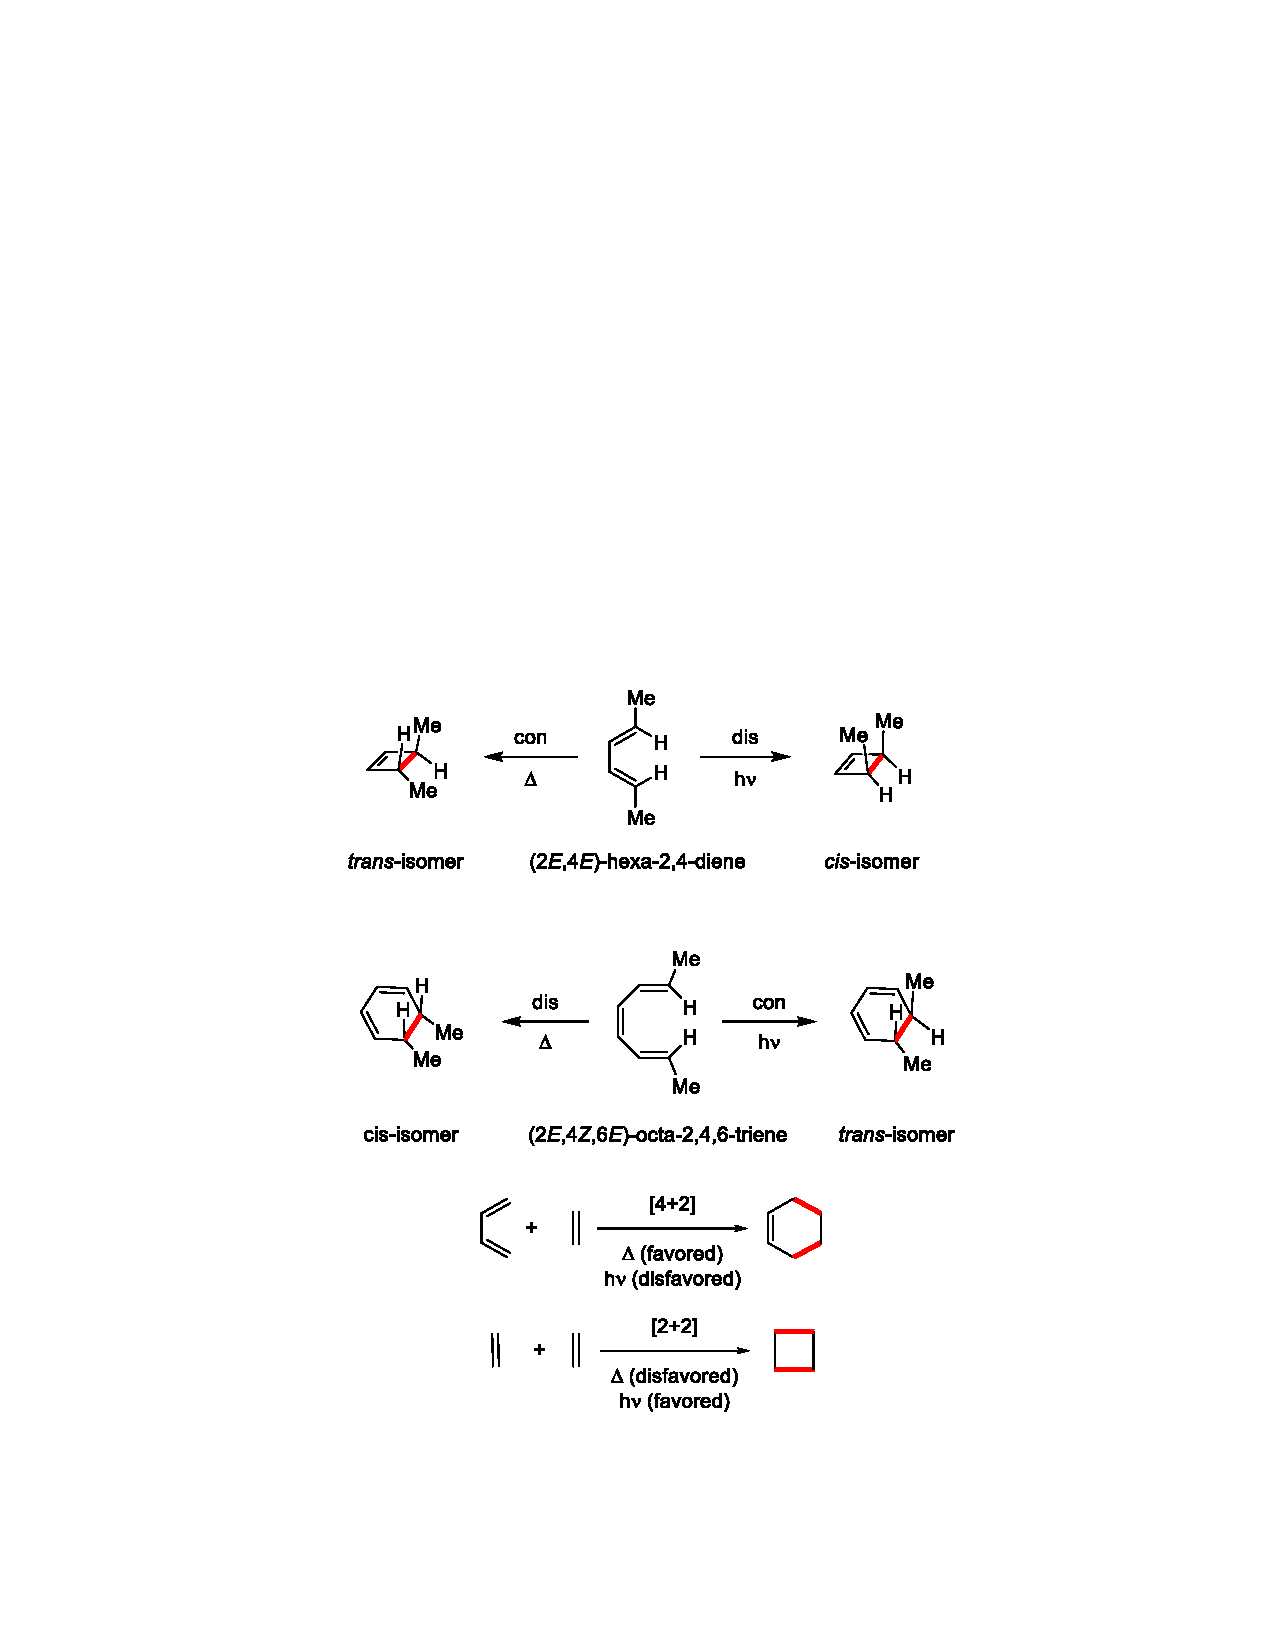
\includegraphics[width=10cm]{./pic/t10-1.pdf}
\end{figure}

\noindent\textbf{10.1.}
化合物\textbf{1}在加热下经一系列环加成反应得到土楠酸\textbf{2},结构如下所示。画出反应的具体步骤并对其中涉及的电环化反应进行分类。

\begin{figure}[h]
	\centering
	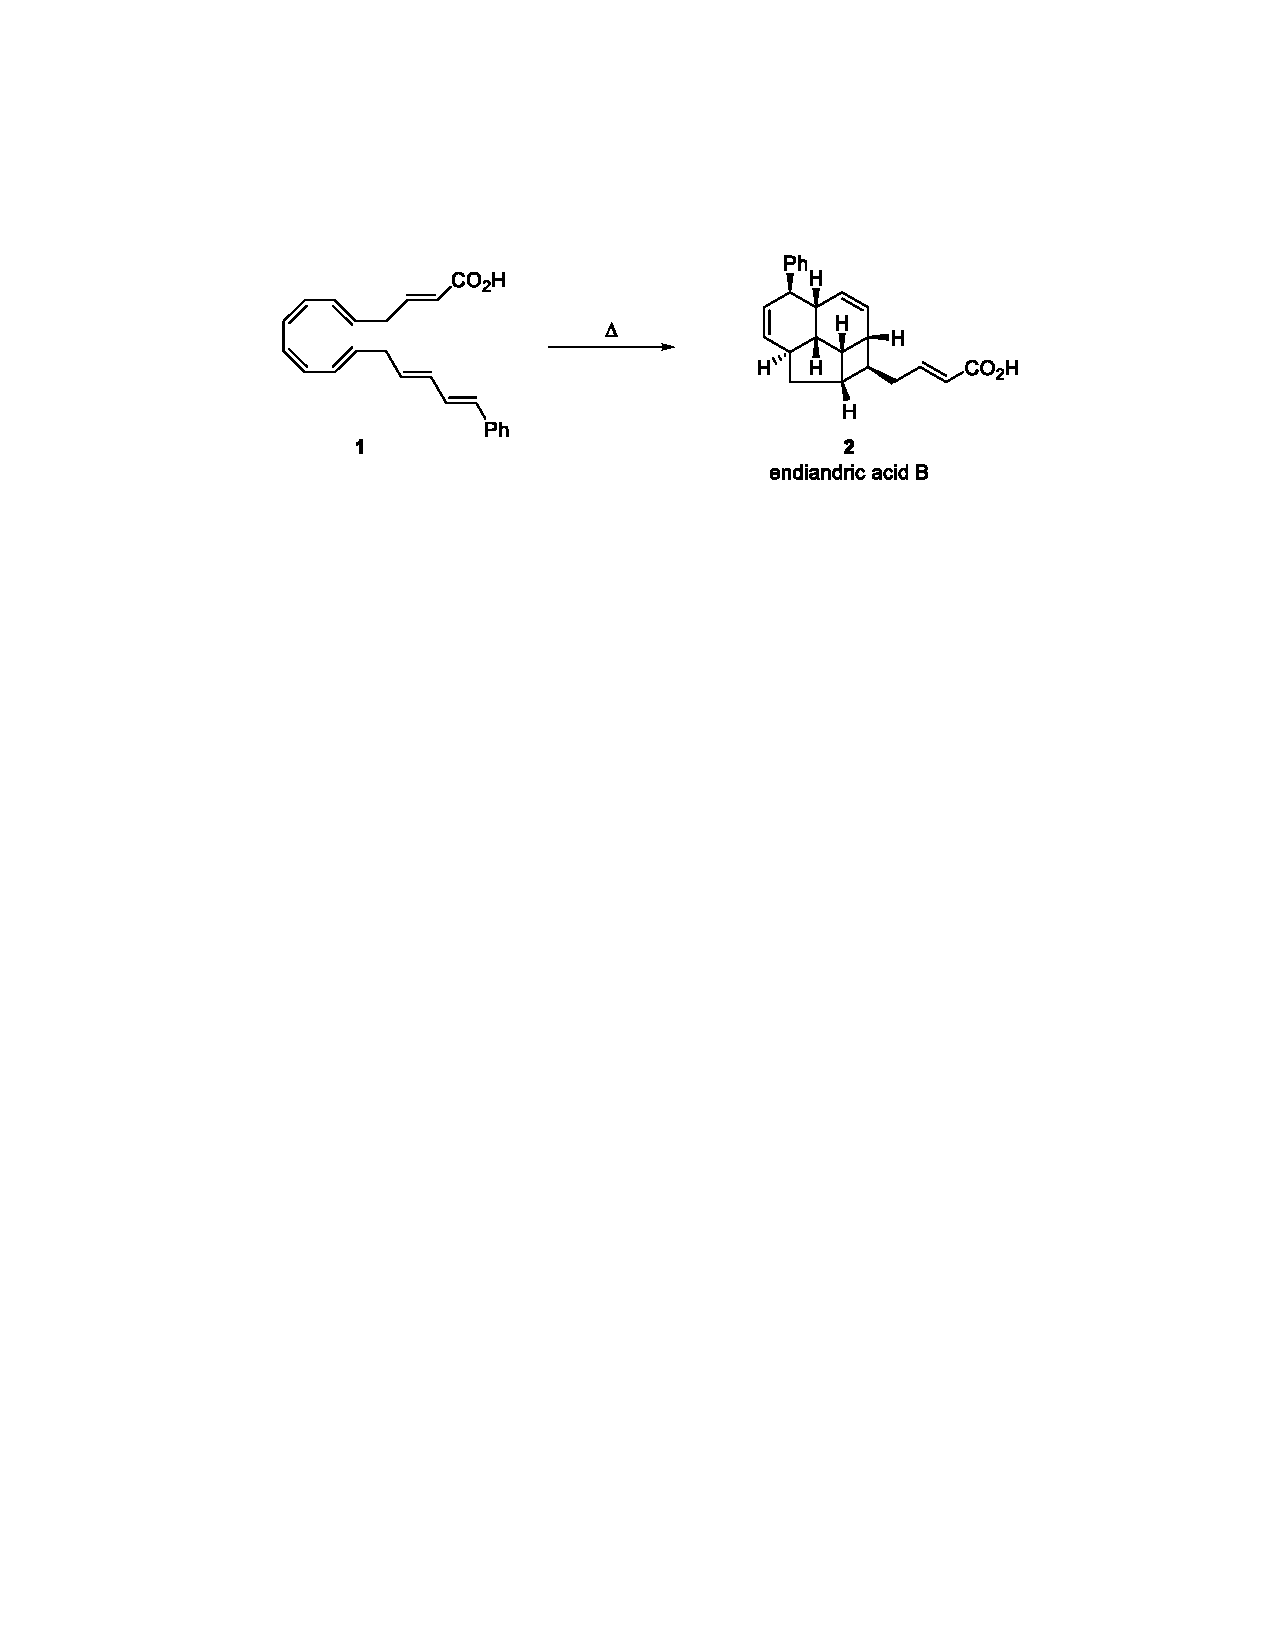
\includegraphics[width=12cm]{./pic/t10-2.pdf}
\end{figure}

在以下两小问的反应中,分别有多少$\pi$电子参与?根据Woodward-Hoffmann规则,这些反应的条件为光照还是加热?

\noindent\textbf{10.2.}

\begin{figure}[h]
	\centering
	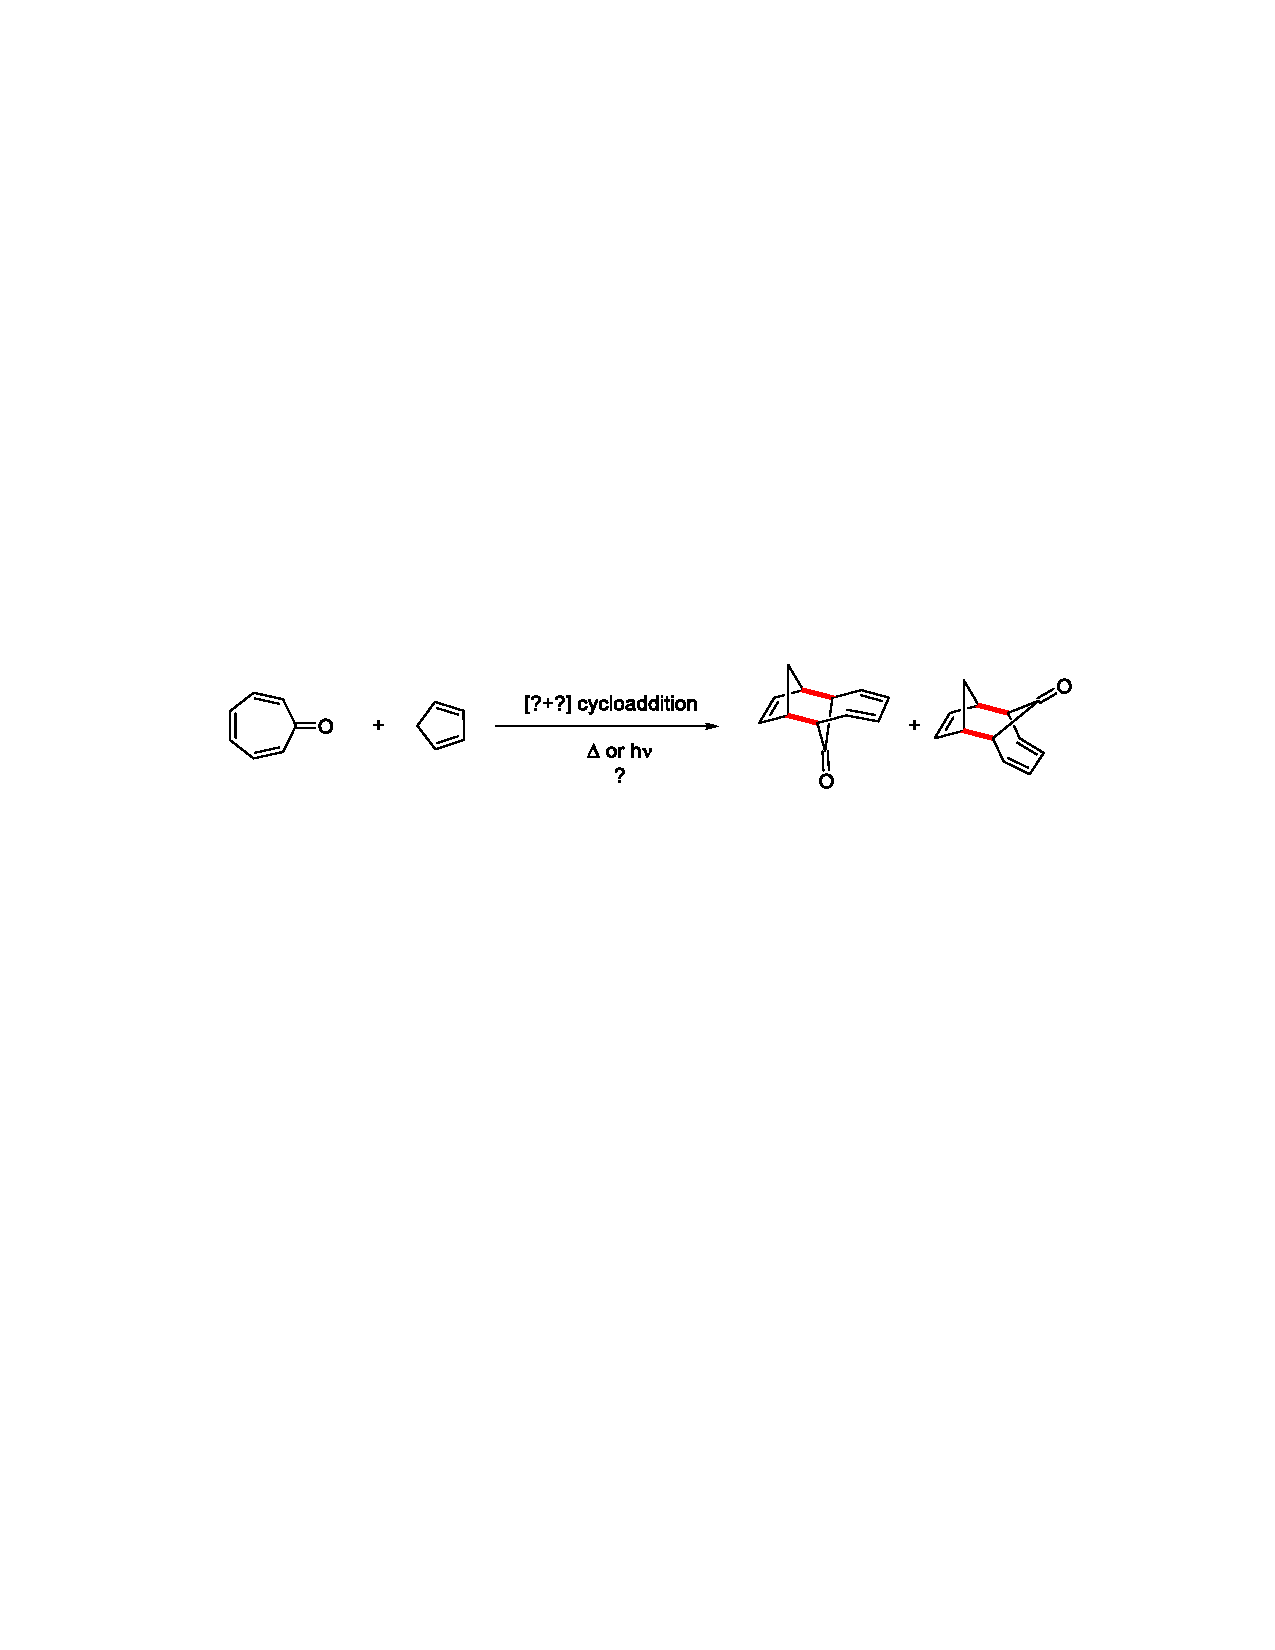
\includegraphics[width=13cm]{./pic/t10-3.pdf}
\end{figure}

\noindent\textbf{10.3.}

\begin{figure}[h]
	\centering
	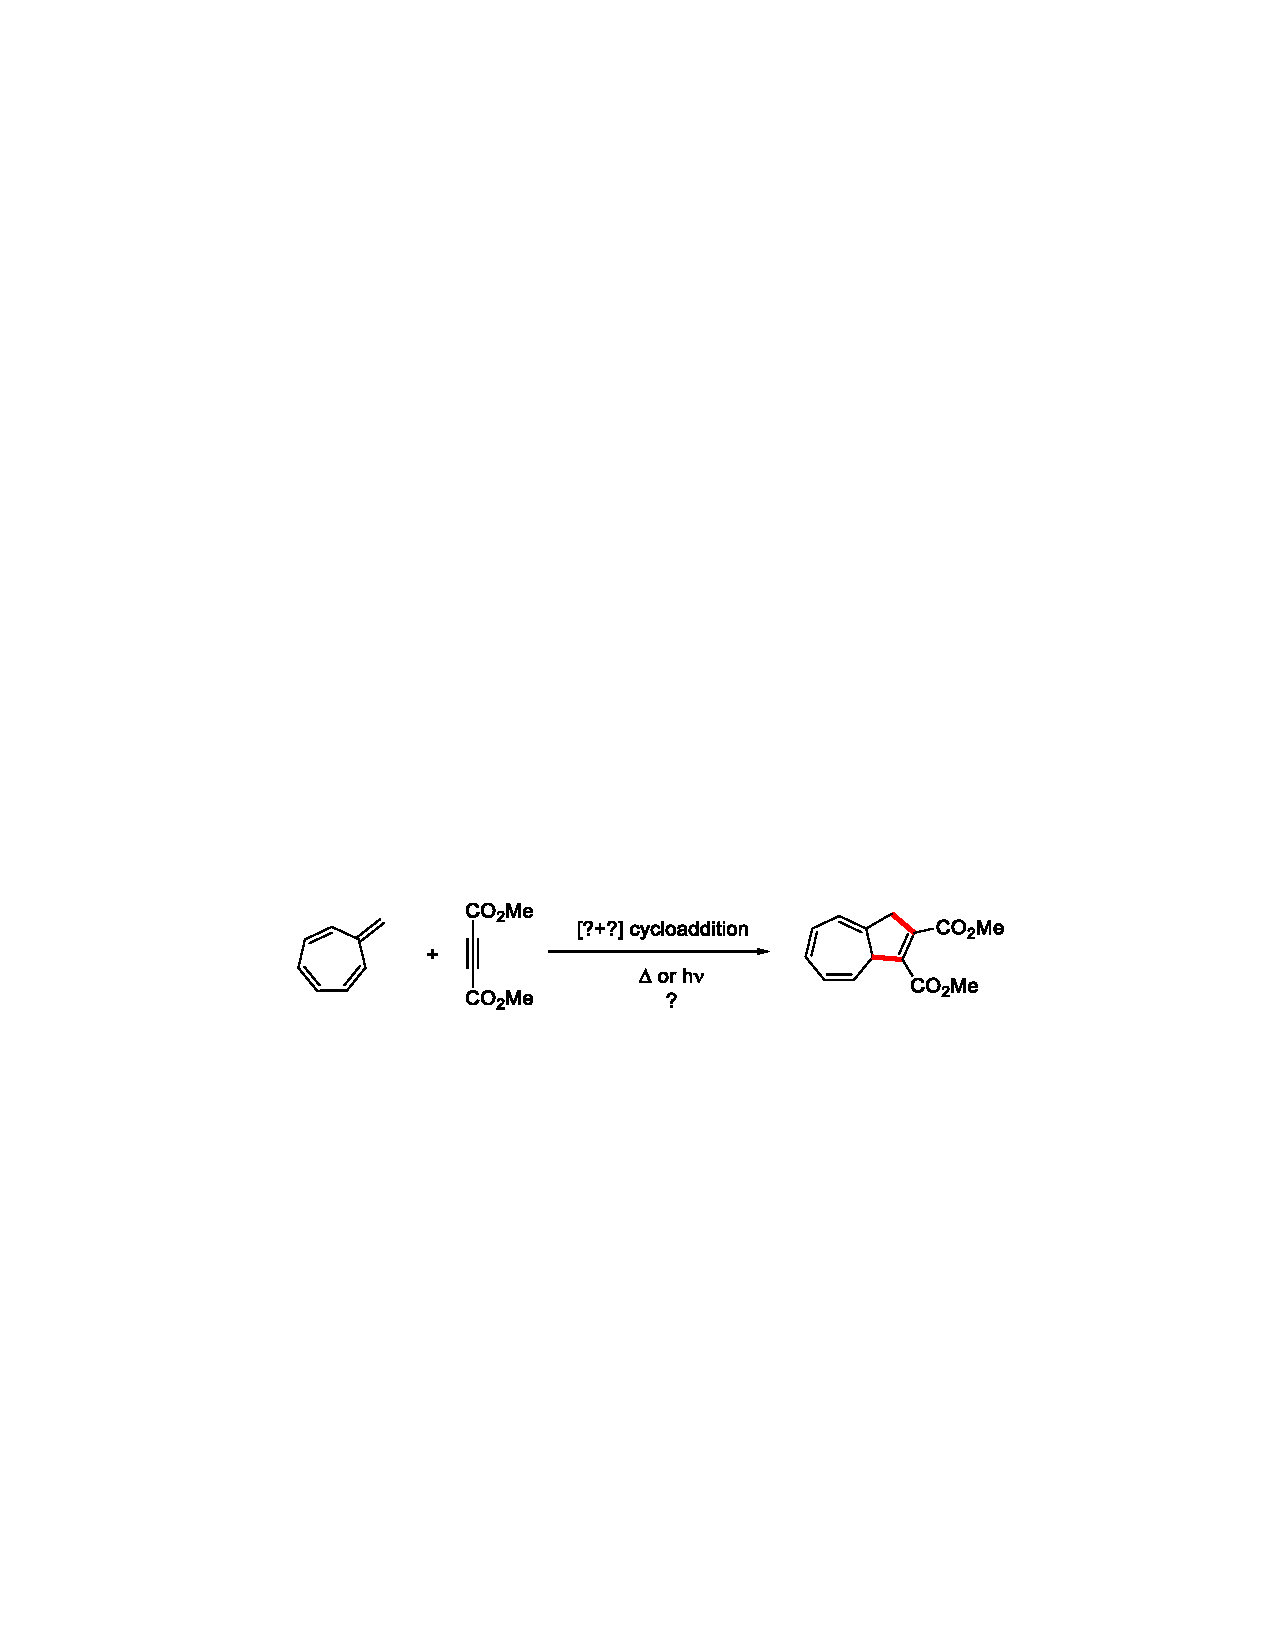
\includegraphics[width=12cm]{./pic/t10-4.pdf}
\end{figure}

\noindent\textbf{10.4.}
\textbf{A}与琥珀酰亚胺可以经连续的Diels-Alder反应生成化合物\textbf{3}。画出化合物\textbf{A}-\textbf{C}的结构。

\begin{figure}[h]
	\centering
	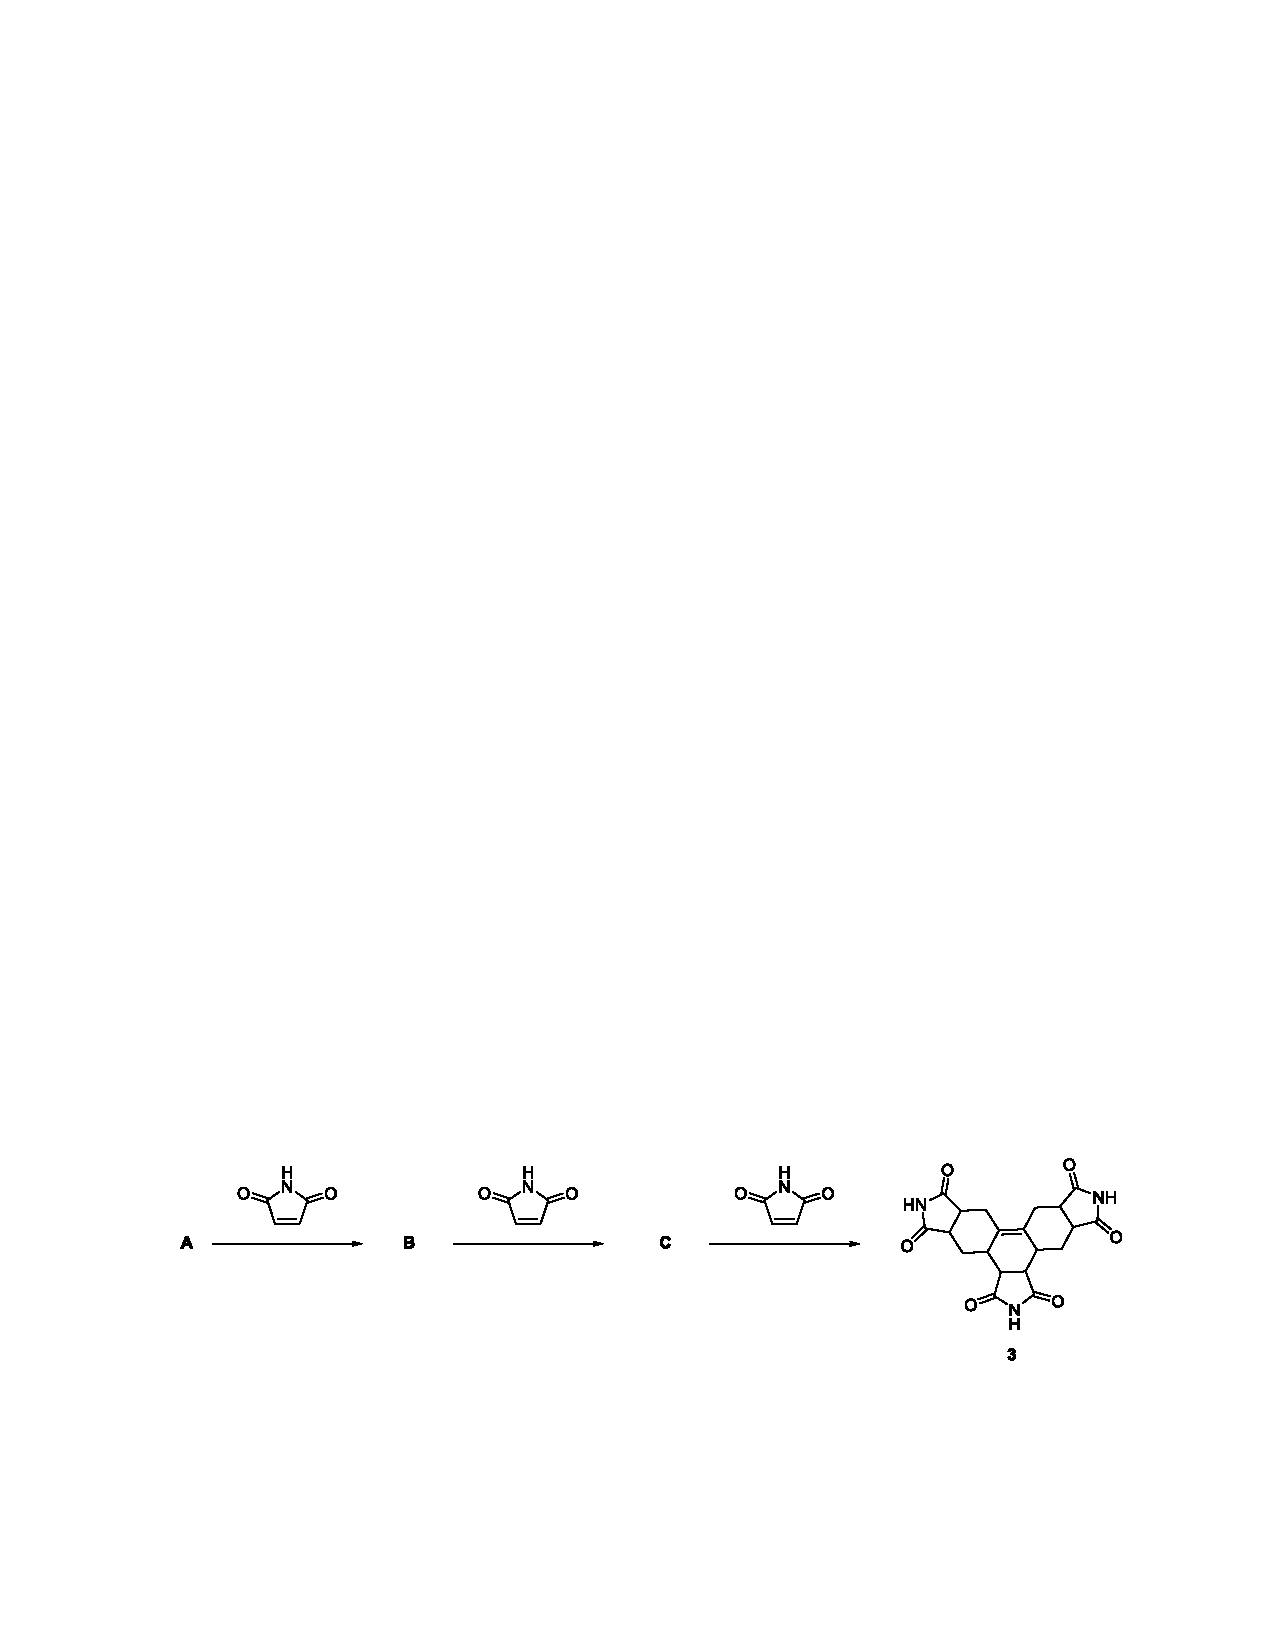
\includegraphics[width=16cm]{./pic/t10-5.pdf}
\end{figure}

\noindent\textbf{10.5.}
下面的反应路径图展示了从邻二甲苯开始合成苯系四环烃\textbf{I}的内式异构体的方法。用四溴代邻二甲苯\textbf{D}与碘化钠进行Br\textsubscript{2}消除反应,产生一个活性中间体\textbf{E},再经历一个4$\pi$电环化获得化合物\textbf{F}。画出中间体和产物\textbf{D}-\textbf{I}的结构。

\begin{figure}[h!]
	\centering
	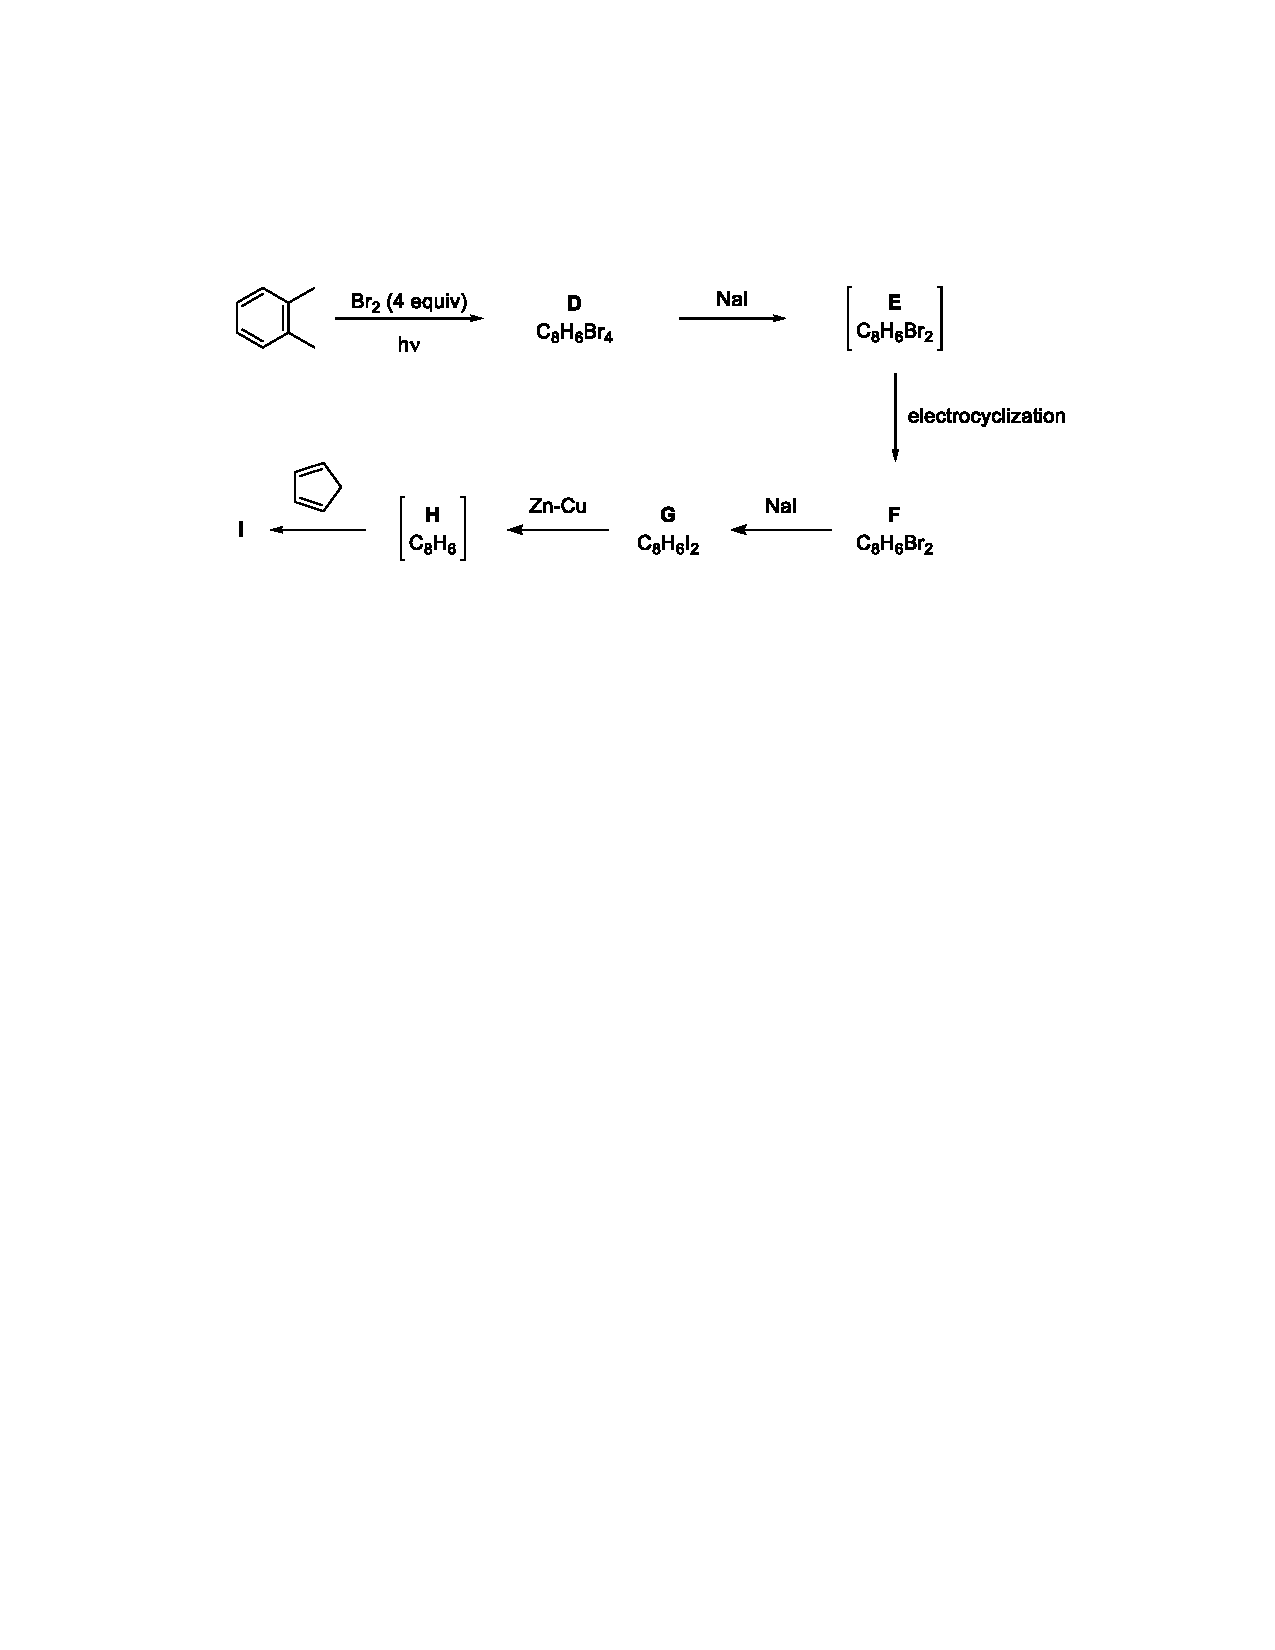
\includegraphics[width=12cm]{./pic/t10-6.pdf}
\end{figure}

\noindent\textbf{逆Diels-Alder反应}

逆Diels-Alder反应是Diels-Alder反应的逆反应,环己烯衍生物分解为二烯及亲双烯体的反应便是一例。一般而言,逆Diels-Alder反应由热引发,但在某些情况下,由于底物性质不同,低温更利于反应的进行。

在有机化学、配位化学中,环戊二烯是常用的合成中间体,未取代的环戊二烯由二环戊二烯的分解反应制得。然而,由于顺式双键易迁移的特点,取代的环戊二烯并不稳定,因此制备取代的环戊二烯的方法十分有限。在下面的反应路径中,展示了取代环戊二烯衍生物的合成方法,其中除了逆Diels-Alder反应,还有反Diels-Alder反应,即富电子的亲双烯体和缺电子的双烯体(如四嗪\textbf{4}),通过亲双烯体的HOMO与双烯体的LUMO的相互作用进行的环加成反应。

\noindent\textbf{10.6.} 画出中间体和产物\textbf{J-N}的结构。

\begin{figure}[h!]
	\centering
	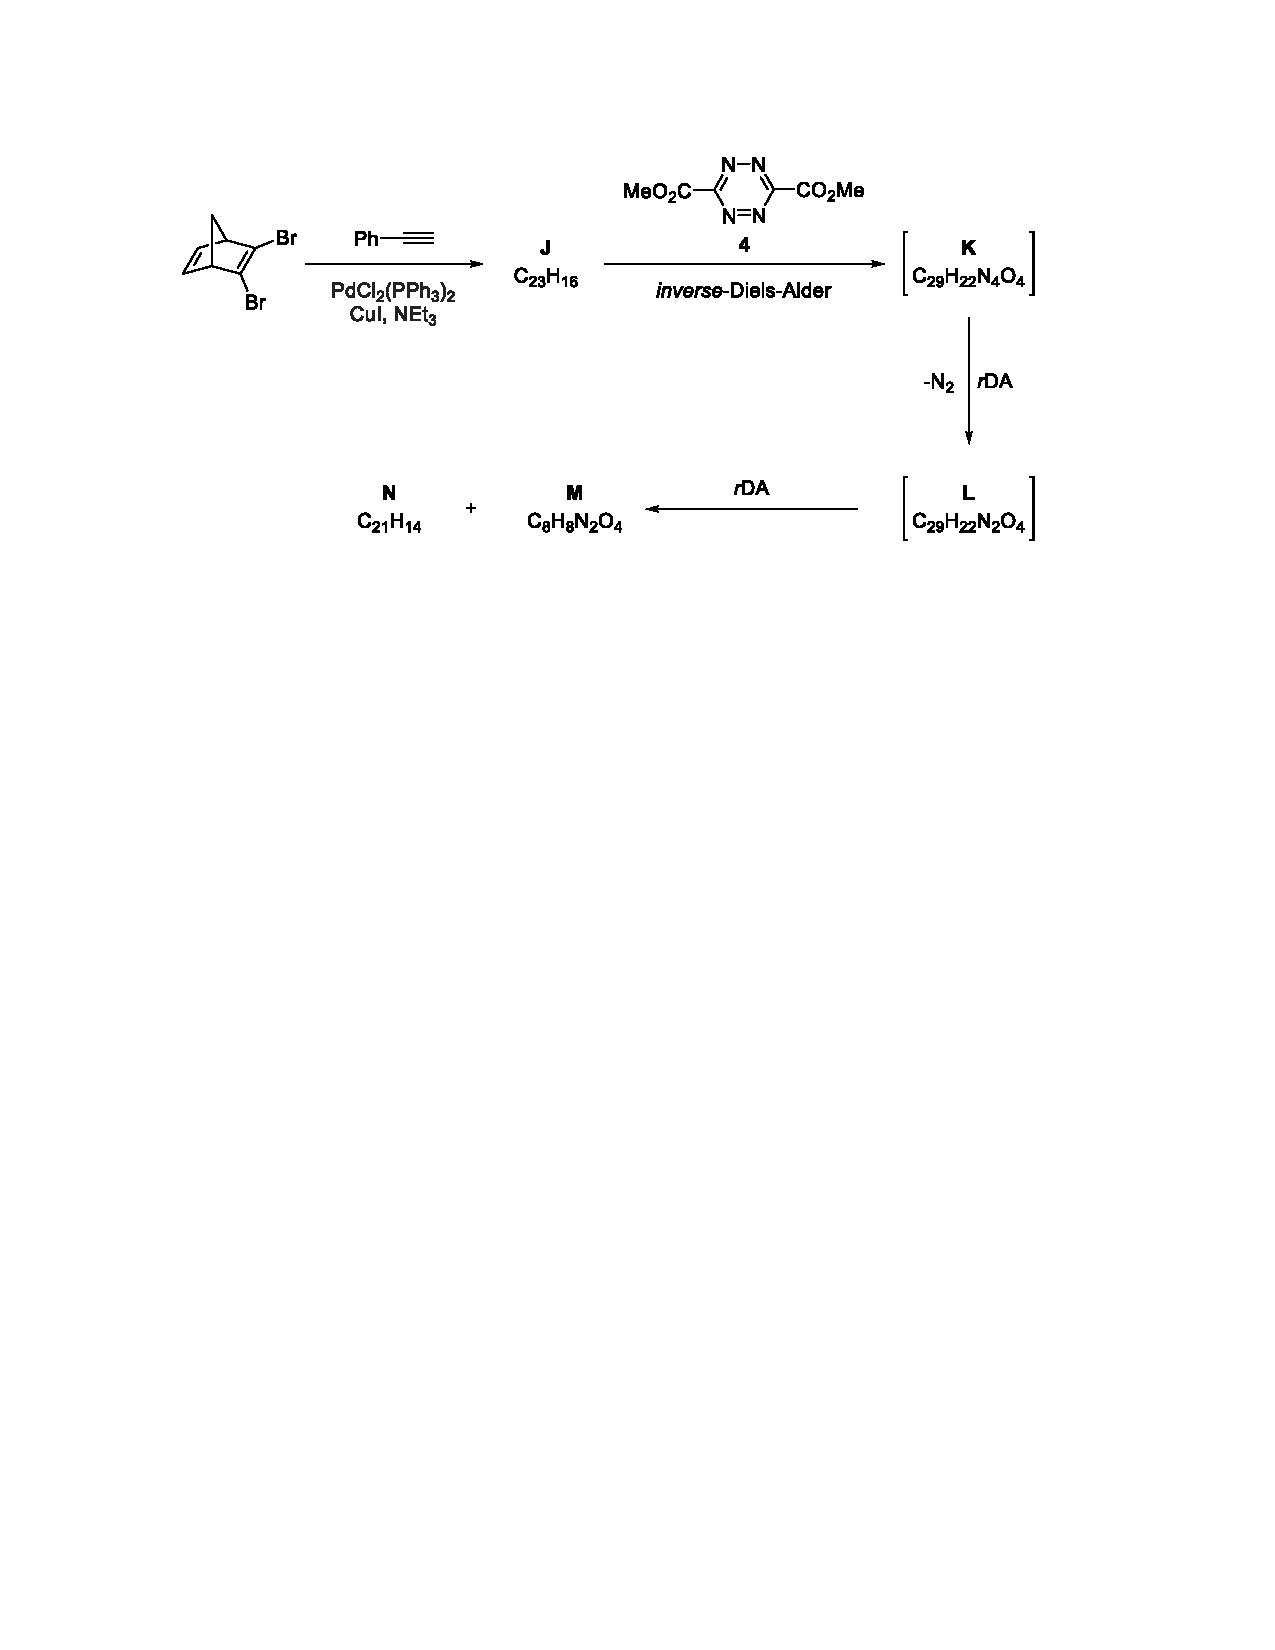
\includegraphics[width=13.5cm]{./pic/t10-7.pdf}
\end{figure}

\noindent\textbf{10.7.}
亲核芳香取代反应是有机合成化学中一类非常重要的反应。在下图中,两种不同结构的芳香卤化物\textbf{5}在不同的反应条件下进行反应,反应中经历了两种不同的中间体,这两种中间体具有环状1,3-二烯结构。画出两种产物(\textbf{O}和\textbf{P})的结构,讨论生成这两种产物过程中的可能中间体。

\begin{figure}[h!]
	\centering
	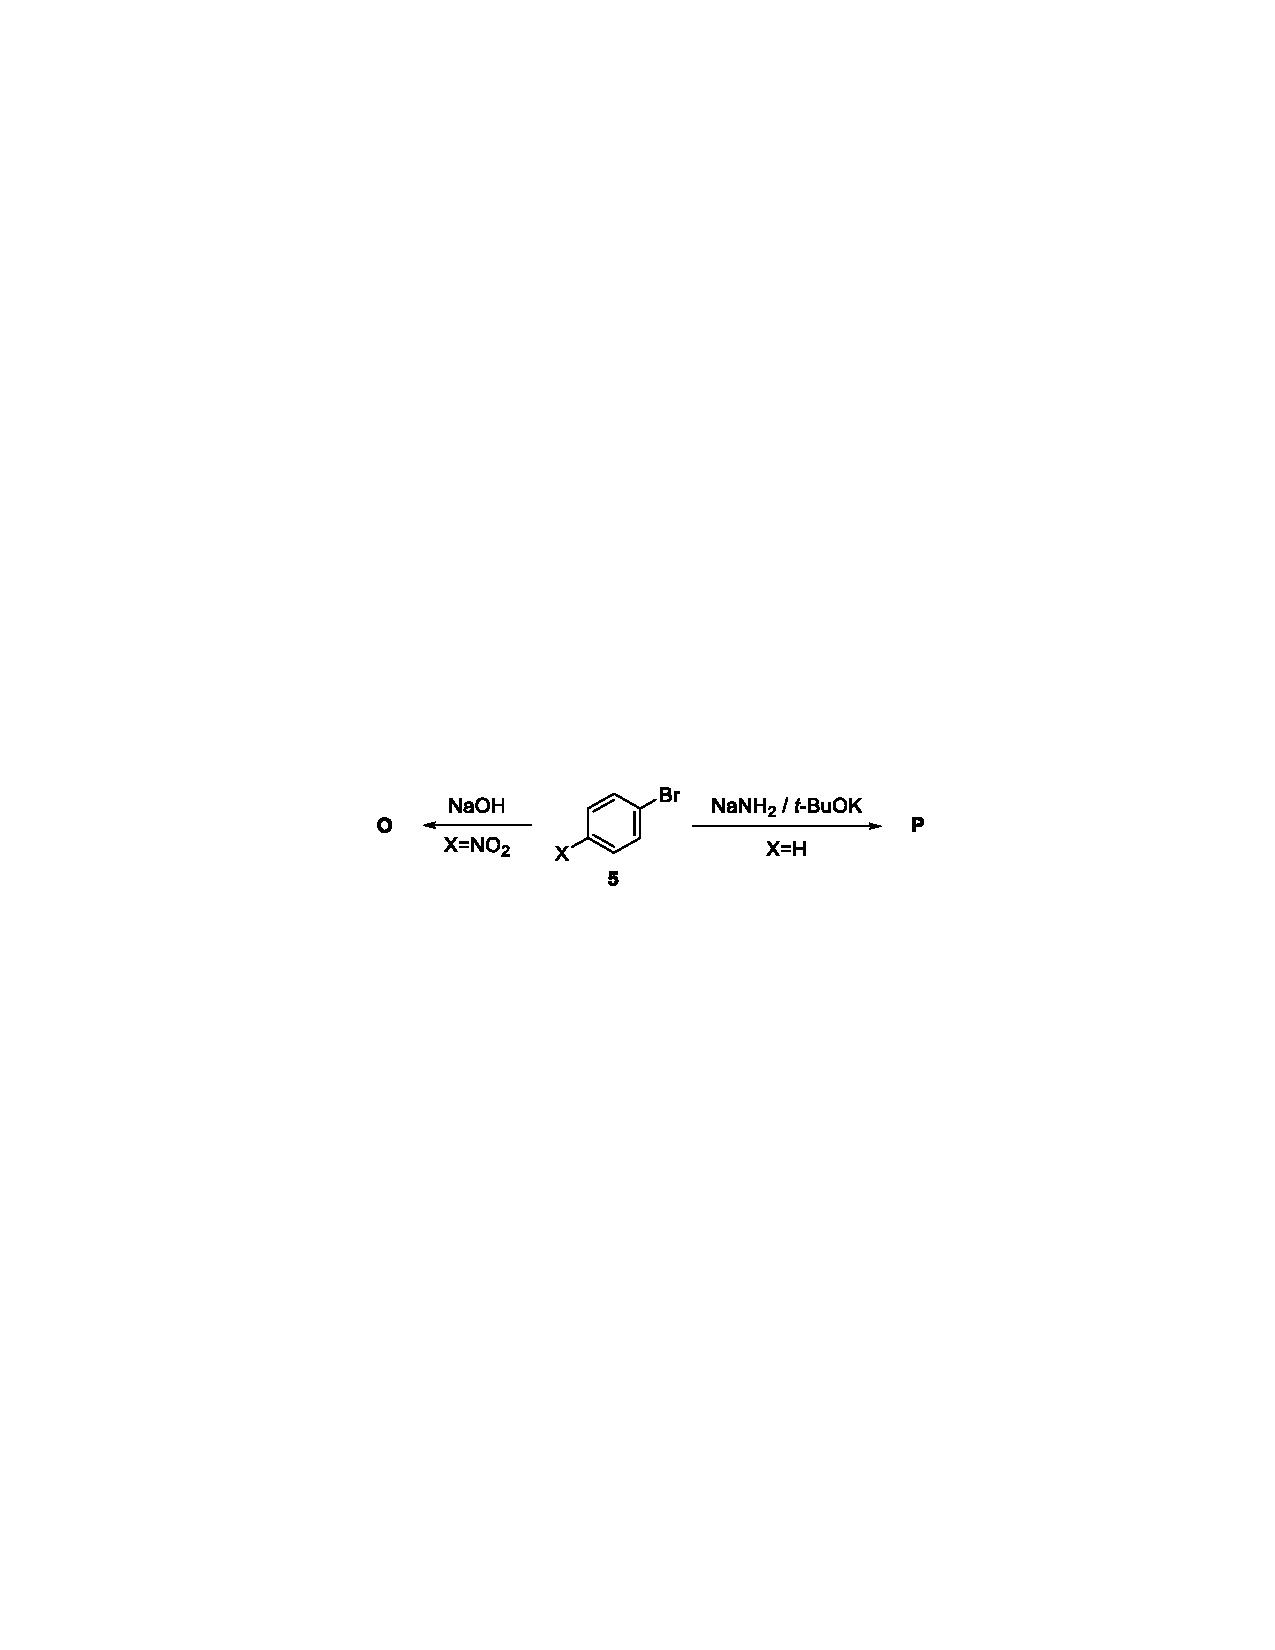
\includegraphics[width=8.5cm]{./pic/t10-8.pdf}
\end{figure}